\documentclass[journal]{IEEEtran}
\usepackage[utf8]{inputenc}
\usepackage{graphicx}
\usepackage[style=numeric, backend=biber, sorting=none]{biblatex}
\addbibresource{references.bib}

\begin{document}
%
% paper title
% can use linebreaks \\ within to get better formatting as desired
\title{Lisp Machines and the Analysis of Their High-Level Language Computer Architecture}

\author{
	\IEEEauthorblockN
		{
			Dominic Dabish and Evan Bradley\
		}
	\IEEEauthorblockN
		{
			\\School of Engineering and Computer Science
		}
	\IEEEauthorblockN
		{
			\\Oakland University Engineering Center, 115 Library Drive, Rochester, MI 48309
		}
	\IEEEauthorblockA{
		\\ \{dadabish, edbradley\}@oakland.edu
		}
\thanks{
This paper was submitted for review on March 25, 2016. It was produced with help from Oakland University's subscription to publication sources with information on Lisp and Lisp machines.
}%
\thanks{
D. Dabish and E. Bradley are Computer Science students at Oakland University in Rochester, MI, 			48309. 
}%
}

% The paper headers
\markboth{Term Paper, CSE~364 - Computer Organization, Winter 2016}%
{Shell \MakeLowercase{\textit{et al.}}: Bare Demo of IEEEtran.cls for Journals}

% make the title area
\maketitle

\begin{abstract}
The high-level capabilities that Lisp affords programmers make the language useful in certain applications, but at the cost of its programs running slowly on most computers, which were designed for different types of executions. To account for the incompatibility between Lisp and the hardware on which it is executed, computers called \textit{Lisp machines} have been designed specifically to run Lisp programs by designing the processor hardware to accommodate the language features Lisp possesses. Achieving greater efficiency in running Lisp was accomplished using various methods, both in the hardware and in how data would be represented in the software. Hardware alterations largely consist of changes to the circuitry in the processor itself, as well as the number and purpose of processors in the machine. Software changes mostly correspond to the representation of lists, the main data structure in Lisp. Lisp machines were largely deprecated in the 1990s, giving way to traditional computers which were fast enough to run Lisp with reasonable speed. Despite this, Lisp machines remain a popular subject for study and discussion amongst those who are familiar with Lisp.
\end{abstract}
% IEEEtran.cls defaults to using nonbold math in the Abstract.
% This preserves the distinction between vectors and scalars. However,
% if the journal you are submitting to favors bold math in the abstract,
% then you can use LaTeX's standard command \boldmath at the very start
% of the abstract to achieve this. Many IEEE journals frown on math
% in the abstract anyway.

% Note that keywords are not normally used for peerreview papers.
\begin{IEEEkeywords}
Lisp, Lisp machine, computer engineering, vintage computing, computer organization.
\end{IEEEkeywords}

\section{Introduction}
The history of Lisp begins with Alonzo Church's introduction of lambda calculus in the 1930s, where Church attempted to reconcile mathematics and computation. Lisp takes many notational cues from lambda calculus, and in a sense, serves as a practical implementation of the ideas Church presented. Lisp machines were created for specific use with Lisp as a response to the decreasing costs and increasing complexity of computers in the 1970s, and were rendered virtually defunct in the 1990s by the same conditions that created them. 

\subsection{Early history of Lisp}
John McCarthy created Lisp while working to create a new computer language to replace languages like the Information Processing Language (IPL) and Fortran, which he saw as cumbersome and insufficient for programming artificial intelligence (AI) \cite{stoyan}. He began work on what was then called lisp LISP, or the LISt Processing language, in 1958 while working at the Massachusetts Institute of Technology (MIT), and published a Communications of ACM paper in April of 1960 that detailed the basic workings of the language he constructed \cite{stoyan, mccarthy}. By April 1958, Steve Russell had implemented some Lisp functionality in machine language on the IBM 704, much to the surprise of McCarthy, who believed his work to be entirely theoretical before seeing the implementation. Development of Lisp began to occur in a more concrete fashion after the actual implementation of Lisp code on the IBM 704. McCarthy and his team then began to focus on creating a usable version of Lisp in addition to creating something mathematically elegant \cite{stoyan}.

In the late 1960s, Jon L. White published a paper describing MACLISP, a variation of Lisp that ran on the Digital Equipment Corporation's PDP-6 \cite{stoyan}. This was followed by the creation numerous other Lisp dialects by individuals and groups who were not directly related to McCarthy. Many of these were combined into Common Lisp in the 1980s. One of these dialects was Scheme, which, along with Common Lisp, continues to be one of the two major Lisp dialects to date. It was created in 1975 by  Guy L. Steele and Gerald Jay Sussman at the MIT AI Lab, and on whole is much simpler than Common Lisp.

\subsection{History of Lisp machines}
The first Lisp machines were released in the mid-1970s and grew in number during the 1980s. They were some of the first single-user workstations, which at the time were an exception to the common timesharing systems where multiple users would connect to a single machine through terminal stations. This change came in part due to Lisp's nature of consuming the entirety of the computer's resources, which made its use difficult on multiple-user systems \cite{andromeda}. Two main companies emerged from the increasing demand for Lisp Machines: Symbolics and Lisp Machines, Incorporated. Larger companies began to produce Lisp Machines as well, including Xerox and Texas Instruments. 

These machines were often seen as valuable for not just their ability to run Lisp, but for the advanced features they offered in terms of graphical user interfaces (GUIs) and programmability due to the flexibility that Lisp afforded programmers. Despite their advances in usability, they were often behind in terms of hardware due to their niche audience, they sold to a much smaller market than general-purpose machines, which quickly raced past Lisp machines in terms of hardware capability \cite{withington}. Eventually general-purpose computers became faster at running Lisp despite the hardware incompatibilities, and in combination with the slow development of AI in the early 1990s, most Lisp Machine vendors either left the market or went bankrupt by the mid 1990s.

\section{The Basics of Lisp}

\subsection{Lists and functions}
Lisp programs are constructed using functions that invoke each other. After the nest of functions are evaluated, it is typical of Lisp programs to evaluate to one final value.

All expressions in Lisps are written in forms. One of the most common forms includes an application of functions. For example, the function call in common mathematics \texttt{g(x)} is represented in lisp as \texttt{(g x)}. In this example, \texttt{g} is the name of the function and the argument(s) follow, with \texttt{x} being the only argument in this example.

Numbers and some other basic expressions such as booleans qualify as \textit{self-evaluating forms}, meaning that those expressions evaluate to the same values.  

\begin{figure}
	\centering
	
\includegraphics[width=3.5in]{Chain}
	\caption{Box-and-pointer diagram representing an example of a sequence chain. This particular chain contains the sequence of the elements d, o, m. The empty box represents nil.}
	\label{Data representation}
\end{figure}

Lisp was built to support complete abstraction of data. Data abstraction can isolate a compound data object and its usage from the fabrics of how primitive data objects are constructed. The reason that data abstraction is necessary is to provide foundation to a program in such a way that tasks can be performed without having information about the data beforehand. This is different from a concrete representation of data, which can be defined independently from the program which will handle said data.

\texttt{car} and \texttt{cdr} are primitive operations that can be performed on lists and other data objects. They are used to both extract from lists and manipulate them.  The car operation extracts the first element from the list, and the cdr operation extracts the rest of the list. For example, consider a list with three elements: \\\\\texttt{'(d o m)}\\\\ The following expression involving the car and cdr operations on said list evaluate to the following: \\\\\texttt{(car  '(d o m))}\\\\ evaluates to \texttt{d}, and \\\\\texttt{(cdr '(d o m))}\\\\ evaluates to \texttt{'(o m)}.\\\\ These are classified as procedures operated on list objects. However, this is not the same case as pairs. When given the following pair: \\\\\texttt{(cons D d)}\\\\ and operating \texttt{car} and \texttt{cdr} on the pair, the evaluation will return to \texttt{D} and \texttt{d}, respectively.

The IBM 704 was built with specific support for splitting the language's 36-bit machine words into four parts. The first and second parts of the word, both 15 bits each, were the \textit{address part} and the \textit{decrement part}, called \texttt{car} and \texttt{cdr}. The last two parts, \texttt{cpr} and \texttt{ctr} were deprecated. Lisp, being originally marketed as a \textit{list processing language}, named \texttt{car} and \texttt{cdr} for acronyms for \textit{Contents of the Address part of the Register number} and \textit{Contents of the Decrement part of the Register number}. Both of these functions take a machine address as the initial argument, then load the word from memory to extract the bits located.

Pairs are useful when building a sequence in Lisp. A sequence is defined as an ordered collection of data objects. Sequences are one of the fundamental building blocks to perform recursive and other useful procedures. As shown in the Figure 1, the sequence d, o, m is represented as a chain of pairs.\\

\texttt{(cons d (cons o (cons m nil)))}\\

There are also procedures that can perform operations on lists. For example, the procedure \texttt{reverse} takes a list as an argument and returns a list with the same elements, but in reverse order. In this example, the s-value \texttt{(reverse '(d o m))} evaluates to \texttt{'(m o d)}.


\subsection{Environments}
Environments are a specific kind of datatype that allows one to define a set of variables that are bound to specific values. The actual datatype for the environment can be implemented in a variety of ways. Using a data-centric approach, we can introduce the environment datatype as follows:\\\\
\texttt{Env :=}\\\texttt{(empty-env) | (extend-env var val Env)}\\\\Each datatype includes constructors and observers, which Lisp enables the programmer to define and construct. An environment is comparable with a dictionary, in the fact that, when using an extractor, the function must search for the variable (word) and, once found, will then be able to extract the value (definition). In Lisp, environments share some of the fundamental properties as the logic units in Lisp machines do.

\begin{figure}[!t]
	\centering
	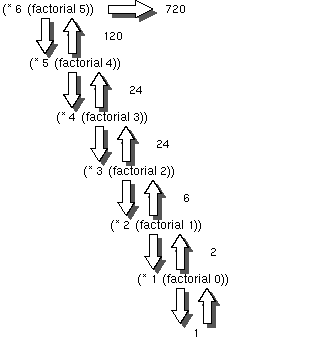
\includegraphics[width=3.5in]{factorial}
	\caption{Diagram of complete recursive evaluation of (factorial 5)}
	\label{Factorial}
\end{figure}

\subsection{Recursion}
Lisp's conventional programming methodology places emphasis on recursion for its uses in environments and lists. Recursive functions are generally defined as functions that refer to themselves in the function-body, with the recursive call argument differing between each step in which the function recurs. A classic example in any programming language is the factorial function. As shown below, the factorial function makes use of a decreasing integer with a base case that enables the program to terminate. \\

\texttt{(defun factorial (n)}\\\texttt{
	(if (= n 0)
	1
	(* n (factorial (- n 1)))))
}\\\\In this example, the program checks if the argument \texttt{n} is equal to 0 (the base case). If so, the function evaluates to 1 and terminates; otherwise, the function will multiply the argument by the factorial with \texttt{n-1} as the argument instead. This creates a chain similar to Figure 2, and evaluates to the factorial of \texttt{n}.

A way in which recursion is commonly used in Lisp that includes list-based manipulation is shown below. In this example, which shows another design pattern that is possible and common in this language, is the \texttt{list-of-all?} function, which has two arguments, a \textit{predicate} and a \textit{list}, and evaluates to the value \texttt{\#t} (true) or \texttt{\#f} (false), based on whether or not the entire list contains elements that satisfy the predicate function requirements. The example below demonstrates how a recursive function manipulates a list until the list empties.\\

\texttt{
	(define (list-of-all? predicate lst)
			(or 
				(null? lst)
				(and (predicate (car lst))
					 (list-of-all? predicate (cdr lst)))))
}\\\\This example evaluates to \texttt{\#t} and terminates given an empty list, which is the base case. Otherwise, it will extract the first element of the list and check the predicate against it. If the check evaluates to \texttt{\#f}, then the function will evaluate completely to \texttt{\#f}, and not check the rest of the list. However, if \texttt{\#t}, the function will check the rest of the list, discluding the first element. This function will therefore terminate when an element that does not match the predicate is found, or when every element of the list has been checked on by the predicate.

\section{Identifiable Problems in the Execution of Lisp Code}
In a 1987 survey of Lisp machines, Andrew Pleszkun and Matthew Thazhuthaveetil concluded there were four main problems engineers needed to address when designing a Lisp machine: function calls, environment maintenance, efficient list representation, and heap performance. There were multiple solutions to some of these problems, and at the time of their survey, methods of improving these aspects in Lisp machines were seen as valuable topics for further research \cite{pt}.

\subsection{Problems in Execution}
Function calling is a significant feature in Lisp due to its recursive nature, and in general is expensive due to the operations that must be performed for an invocation or return. In particular is the problem of dealing with variables, which must be accessed in a way that costs a minimal amount of time, due to the high frequency with with functions are accessed. Another key component is the versatility of functions in Lisp, which in some cases can contain different types of arguments, a variable number of arguments, and can sometimes be passed as arguments themselves \cite{pt}.

Integral to the problem of function calling is that of maintaining the environment associated with each function. The current environment, which contains the set of variables within the function and their associated values, is changed every time a function is called. As a result, the environment that exists outside the body of the function must be stored during the function's execution, which is not necessarily difficult, but must be implemented in such a way that it is fast. A more complicated problem is that of accessing variables outside of the function, which are contained in other environments. This is called the funarg problem, which presented difficulties to McCarthy and his team even before it became a focus for Lisp machine engineers \cite{stoyan, pt}.

Lists are the primary data structure of Lisp, and as such a significant portion of execution time in a Lisp program is spent traversing these lists. Therefore, reducing the time require to traverse a list is seen as an important goal in creating a machine optimized to run Lisp. A critical component in achieving this is efficiently determining how data should be handled, which is checked at runtime due to Lisp's lack of typed variables. This is often done through tagging the type of data referred to in the list, typically through hardware solutions \cite{pt}.

Coupled tightly with the management of lists is the heap, which contains all of the referenced Lisps in a Lisp program and holds them in memory \cite{pt}. Garbage collection is the primary solution that Lisp uses to ensure proper memory management without burdening the programmer, but efficient garbage collection is challenging, and presents a difficulty in both hardware and software implementations.

\subsection{Solutions in Lisp Machines}
In their survey, Pleszkun and Thazheuthaveetil found three different general approaches to Lisp machine design, which in turn affected how these problems were solved. The first class of machines contain processors that were not altered on a hardware level, but in the microcode. The second class contains multiple processors that each have specific functionality to assist in executing Lisp code. The third class contain multiple identical processors and function by executing multiple functions in a program concurrently. They call these distinctions Class M, S, and P machines, respectively \cite{pt}.

In solving the problem of evaluating the arguments of functions the Class M and Class S machines will typically allow for code to be run in different formats, the fastest being a compiled code that tags the arguments types and largely bypasses the evaluation process, and the slowest being interpreted code that runs them directly. The Class P machines attempt to solve this through passing each argument to a different processor for evaluation, and in the case one one machine, even allowing incomplete results to be sent to encourage further parallel execution \cite{pt}.

Two primary implementations of the environment are called \textit{deep binding} and \textit{shallow binding}, which serve as variations on a linked list of name-value pairs of functions and referencing contexts of variable associations. Deep binding makes use of a simple linked list of name-value pairs that is searched every time the function is called, and in the worst case the entire list must be traversed. Shallow binding uses a table that holds the name-value pairs. While this allows for faster function calling, the values in any variables that are overwritten have to be stored elsewhere while the function executes.

While lists function quite well as a way of mathematically representing data, they can be computationally inefficient. Therefore, some Lisp machines have represented them in more compact forms, which the authors classify as \textit{vector-coded} and \textit{structure-coded}. Vector-coded representations assume that a list is linear, or that none of its elements are themselves lists. Making this the default case speeds up the evaluation of list elements, with elements that point to other objects treated as exceptions that will evaluate slower. Structure-coded representations attach tags to each list cell that identifies its place in the list. This information allows the list to be traversed quickly, and allows for fast access to individual cells. The implementations of each of these representations vary from machine to machine, as there are multiple implementations of each \cite{pt}.

Additionally, tail recursion is a common programming technique and design pattern to follow that increases speed tremendously, and decrease memory usage. Using traditional recursion, typically calling the function recursive is preceded by calculations. Consequently, the final evaluation is dependent on the complete transaction of the recursive calls. However, when using tail recursion, the calculations are all completed prior to executing recursive calls. Tail recursion takes the evaluation of the current step before passing it into the next recursive step. It is more optimal due to the fact that the current memory allocation is then no longer required.

Lisp delegates the management of the heap to the system rather than the programmer, which necessitates the need for an algorithmic method in which heap data can be allocated when needed and deallocated when it is no longer wanted. The limited amount of memory available to systems has made the reclamation of used space the most researched aspect of heap maintenance, which is commonly referred to as \textit{garbage collection}. Garbage collection is a two-stage process: the system must first identify memory locations that should be reclaimed, and then must simply identify them as such. Two common methods of garbage collection were present in most Lisp systems: \textit{reference counting} and \textit{marking}. Reference counting consists of keeping a list of the number of references for each object in the code and marking it as free space once that number goes to zero, but suffers from numerous drawbacks, such as the memory requirement of keeping such a list. Marking is more common in Lisp machines, and consists of marking each object with a one-bit field to indicate whether it should be removed. Once all available heap space has been allocated, any the memory cells containing objects marked for reclamation are overwritten.

\section{A Proposed Lisp-Based Processor by Steele and Sussman}
In March 1979, Steele and Sussman, researchers at the MIT AI Lab in the 1970s, outlined and discussed a processor that they suggested would allow for the efficient execution of Lisp programs under a dialect of Lisp they had created \cite{ss}. While it is uncertain whether their ideas were directly implemented in an actual Lisp machine, they provide solutions to the environment maintenance and efficient list representation problems proposed by Pleszkun and Thazhuthaveetil, providing a great degree of detail in describing their implementation.

The proposed processor would run a simplified version of Lisp, called Scheme, that is a minimal Lisp dialect without many of the compatability features of other dialects, such as Common Lisp. The representation of data structures in Lisp and how the program is traversed are of particular concern, as Lisp's code is itself a data structure. Therefore, their processor is built specifically for traversing the Lisp data structure in an efficient manner. To achieve this, they wrote a Lisp interpreter which functions recursively, operating on a small set of registers to hold pointers to a list memory system which holds the stack for the program's state information between procedure invocations. The evaluation component of the interpreter uses five global variables that simulate registers in a normal machine to hold different components of the program's state. They describe this system as a state machine implementation where the program moves between states as procedures are invoked \cite{ss}.

To reduce evaluation times for atoms and lookup times for variables, the representation of list data is altered slightly so that each pointer contains a field that specifies how the data should be handled. This happens at compilation time, such that the code does not be modified to include these types, and the compiler will appropriately tag the data \cite{ss}. Refer to Figure 1 for a graphical representation of this format generated from a small code sample.

\begin{figure}[!t]
	\centering
	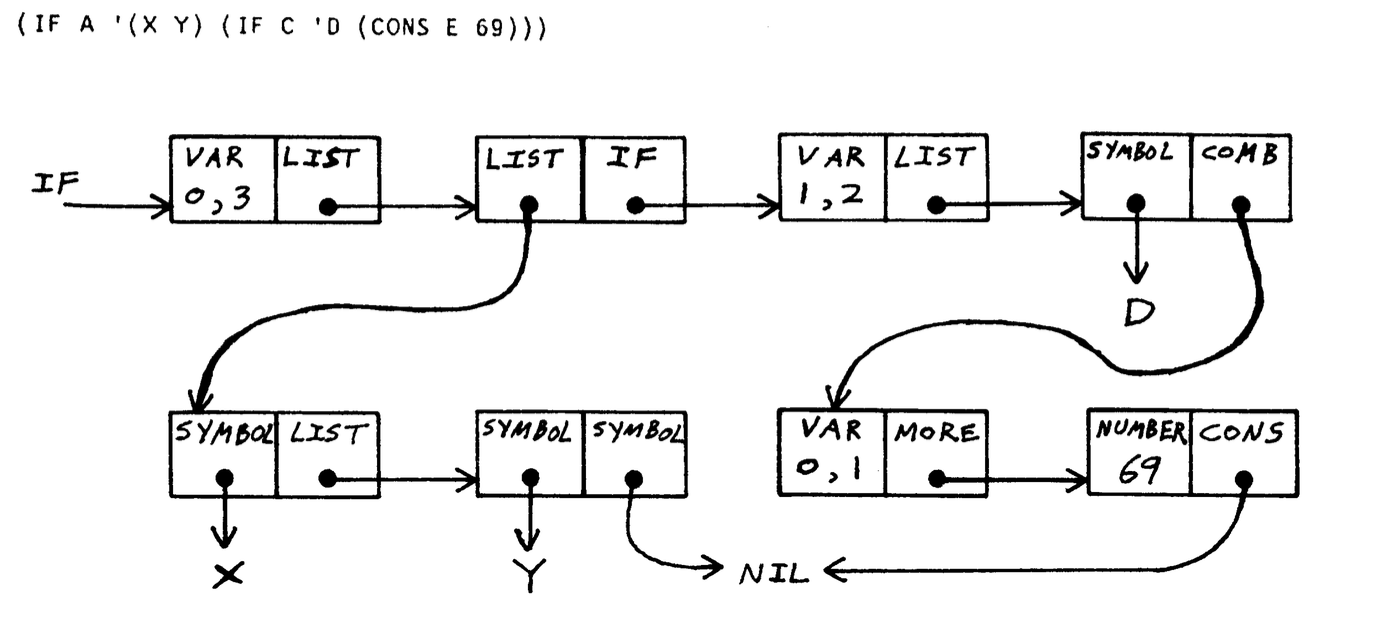
\includegraphics[width=3.5in]{SS_Data_Representation}
	\caption{Example of the tagged data representation used in the Steele an Sussman processor, intended to improve evaluation and lookup efficiency \cite{ss}.}
	\label{Data representation}
\end{figure}

\begin{figure}[!t]
	\centering
	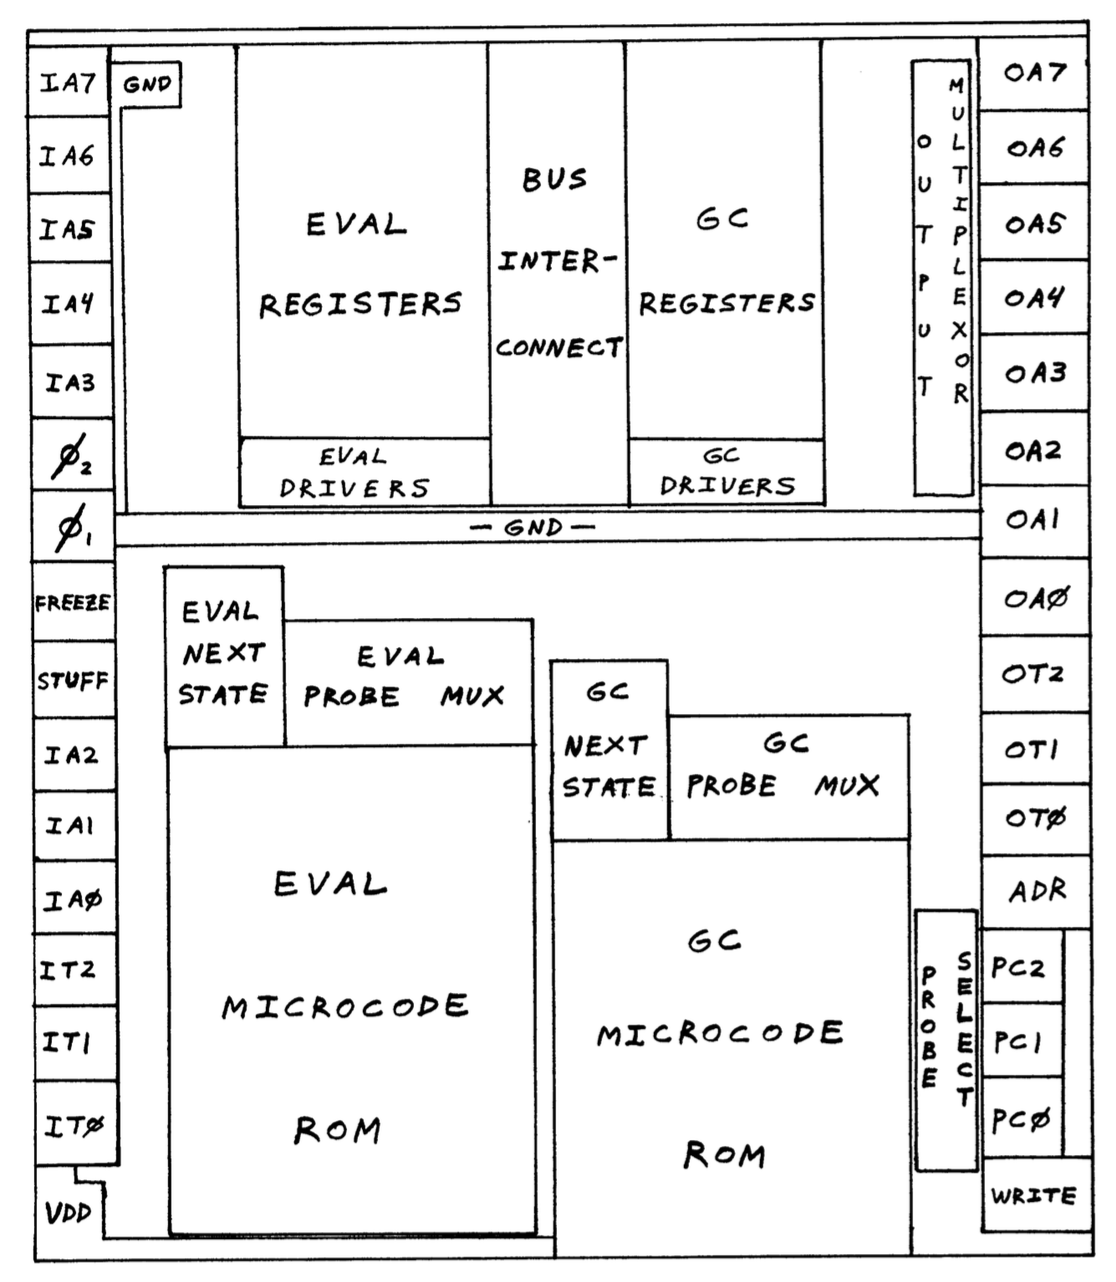
\includegraphics[width=3.5in]{SS_Processor_Diagram}
	\caption{An overview diagram of the processor design proposed by Steele and Sussman. This design was fabricated to test the author's proposed system, but was likely never implemented commercially \cite{ss}.}
	\label{Data representation}
\end{figure}


In their paper, the authors propose that, by combining these two ideas, an efficient interpreter can be designed directly into the hardware. The hardware itself is only concerned with the traversing of the Lisp structure, and so all data is accessed through pointers to memory, which are stored in the processor's registers. Commercially-available memory was only available in a form that stored linearly-indexed vectors rather than linked-lists at the time, so a storage manager was needed to interface between the memory hardware and the processor to ensure the processor could properly utilize the memory. The registers in the proposed processor would hold an 8-bit address and 3-bit type value for each pointer \cite{ss}.

A physical layout was given for this processor, wherein the evaluator and storage manager exist in the form of microcode implemented on read-only memory with a register above each functioning as a form of program counter. Above these are the registers for each unit connected by a bus to transfer information between them. The input connections are supplied on the left and output connections supplied on the right \cite{ss}. A diagram representing the layout of their processor is displayed in Figure 4.

As noted by Steele and Sussman, their processor does not include a meaningful arithmetic logic unit (ALU), and so can not be independent in a system that needs to process real data. However, it contains basic structures for logic and can perform incrementation, and contains the necessary components to run any Lisp program in the described style, due to the simple nature of their proposed Lisp dialect. It is suggested that any actual calculations be done with modules closer to the memory, which most likely contain processors with more sophisticated ALUs \cite{ss}. As such, Lisp machines which implemented designs similar to this would likely take the form of a multi-processor system.

\section{Applications, Obsolescence, and Legacy}
The most popular domain for Lisp machines was  artificial intelligence areas.  This is because the Lisp machines were vastly well developed and generated code that ran efficiently, and allowed programmers to create levels of abstraction that can be specific to a certain domain and create their own infrastructure within the language. Lisp allowed for dynamic creation of new objects, and one of the first machines to support dynamically-sized lists and have a garbage collector that is completely automatic. One of the Lisp machines' main selling points is that there was no need to recompile any of the functions while the program is running, but on-the-fly changes were possible using the language and machines.

In the beginnings of the digital revolution and the dawn of personal computing, some desktop computers were able to run Lisp programs at equal or faster speeds than Lisp machines, and at much cheaper costs. Desktop machines, unlike Lisp machines, had no need for special purposes hardware, which allowed them to be used for non-Lisp applications and made their development and production considerably cheaper. This caused most Lisp machine manufacturing companies to close, and businesses would thereafter cease to create Lisp machines or improve their designs.

Lisp continues to be a popular tool for both education, research, and general programming. \textit{The Structure of Implementation of Computer Programs}, commonly referred to as \textit{SICP}, uses a Scheme variant and is taught at universities nationwide and used by other students for self-learning. Lisp also sees minor use in the general computing market. Paul Graham, co-founder of Y Combinator, used it to create Viaweb, and wrote about the advantages it offered him in keeping ahead of his competitors in an essay written a few years after he sold the company to Yahoo in 1997 \cite{graham}. Though Lisp machines are no longer a commercial enterprise, the continued interest in Lisp and a general interest in retro-computing has kept recreational interest in Lisp machines steady even years after the last manufacturers ceased to exist.

\printbibliography

% that's all folks
\end{document}